\documentclass[a4paper]{article}
\renewcommand{\rmdefault}{ftm}
\usepackage[14pt]{extsizes}
\usepackage[utf8]{inputenc}
\usepackage[russian]{babel}
\usepackage{setspace,amsmath}
\usepackage{graphicx}
\usepackage[left=25mm, top=15mm, right=10mm, bottom=25mm, nohead, footskip=10mm]{geometry}
\begin{document}
\begin{center}
\hfill \break
\large{\textbf{ФГБОУ ВО«Московский Политехнический университет»}}\\
\hfill \break
\hfill \break
\hfill \break
\hfill \break
\hfill \break
\hfill \break
\hfill \break
\large{Лабораторная работа№6}\\
\footnotesize{Файлы\\
Задание 1,2,3\hspace{3cm}Вариант№27\break\\
По дисциплине:\\
Основы Программирования
}
\end{center}
\hfill \break
\hfill \break
\hfill \break
\hfill \break
\hfill \break
\hfill \break
\hfill \break
\hfill \break
\hfill \break
\hfill \break
\normalsize{ 
\begin{tabular}{ccc}
\hspace{4cm}Выполнил & Шукуров Ф.Ф  & группа 181-362\\
\\
\hspace{4cm}Проверил & \underline{\hspace{3cm}}& Никишина И.Н
\end{tabular}
}
\hfill \break
\hfill \break
\hfill \break
\hfill \break
\hfill \break
\hfill \break
\hfill \break
\hfill \break
\hfill \break
\hfill \break
\hfill \break
\hfill \break
\begin{center}\texttt{Москва 2018}\end{center}
\thispagestyle{empty}

\newpage
Лабораторная работа№6;
\\
    \begin{lab1}
        \begin{center}\underline{\hspace{6cm}}\\
            Задание:\\
        \hspace{1cm}Выполнить корректировку программ, написанных для лабораторных работ №1,№4,№5, с таким условием,что бы ввод данных и вывод результатов работы осуществлялся с использованием файлов.
        \end{center}
    \begin{description}
        Описание программы:\\
        \small{Программа была написанна на python 3.6, реализованна в среде os Linux, отвечает за ввод данных, вычисление и вывод данных на экран. Импорт ранее уставноленного модуля \underline{numpy}, а так же, \underline{random}, \underline{math}.}
    \end{description}
    \begin{algoritm}
        Описание Алгоритма:
        \small\begin{enumerate}
            \item Импортируем все необходимые модули.
            \item Используя в блоке чтения файла <<with open ('...','w') as #name>> где 'w' (см.ниже в таблице)\\
            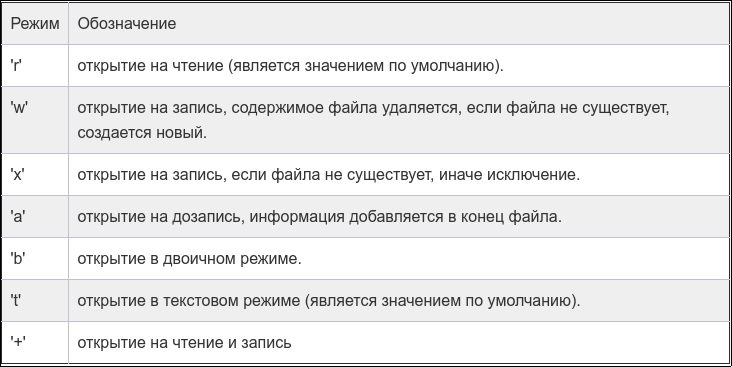
\includegraphics[width=100mm,scale=0.5]{open_func.png}
            \item Будем извлекать нужные числовые значения из файлы с помощью модуля срок:\\
            n = inputs.readline()\\
            n = int(’’.join(n for n in n if n.isdigit()))\\
            где n ~-- переменная, inputs ~-- название перемнной присвоенной в начале блока <<with open(...) as inputs>>, а функция isdigit() ~-- проверка на наличие числа в строчке.
            \item Создаем нужные функции, с блоками проверки внутри нее (см. лабораторные работы №(1,5,4)), а результат записываем в файл \textsc{result}
            \item вызываем функции
        \end{enumerate}
    \end{algoritm}
        \texttt{Листинг Программы:}
    \begin{verbatim}
# -*- coding: utf-8 -*-
import numpy as np
import random, math
from math import log, tan, pi, sqrt
def apend(result):
    with open(r'/home/alan/Files/YandexDisk/programming/programs/
    labs/lab_6/result.txt','a') as apended_text:
        apended_text.write(result)
def lab_1():
    try:
        z1 = a**(sqrt(log(a,b)))-b**(sqrt(log(b,a)))+tan(a*b+(3*p
        i/2))
        z2 = tan(a*b+(3*pi)/2)
        apend(result=("Z1 = " + str(z1) + "\n" +"Z2 = " +
        str(z2)))
    except:
        print('ОДЗ!')
def lab_5():
    sum_or_subtraction = None
    matrix_a = np.random.randint(100, size=(n,m))
    matrix_b = np.random.randint(100, size=(n,m))
    try:
        if output == "1" or output == "+":
            matrix_c = matrix_a + matrix_b
            sum_or_subtraction = " \n+\n "
        elif output == "2" or output == "-":
            matrix_c = matrix_a - matrix_b
            sum_or_subtraction = " \n-\n"
        apend(result=("\n________________\n"+ str(matrix_a) + 
        "\n"+ sum_or_subtraction + "\n" + str(matrix_b) + 
        "\n\n=\n\n" + str(matrix_c) + 
        "\n________________\n\nЗадание№2\n________________\n"))
        transpose_matrix_a = np.transpose(matrix_a)
        apend(result=(str(matrix_a) + "\n\n" + 
        str(transpose_matrix_a)))
    except:
        apend(result='\nОшибка ввода.')
def lab_4():
    massive = []
    massive_absol=[]
    result1=0
    result2=1
    try:
        if y > math.fabs(5):
            123
        else:
            for i in range(massive_quantity):
                massive.append(random.randint(-5,5))
            if y not in massive:
                massive.remove(massive[random.randrange(massive_q
                uantity)])
                massive.append(y)
            for i in massive:
                massive_absol.append(int(math.fabs(i)))
            for i in massive_absol:
                if i < y:
                    result1+=i
            for i in massive_absol:
                if i > y:
                    result2*=i
            if result2 == 1:
                result2 = "Max."
            apend(result=("\n________________\n\nЗадание№3\n_____
            ___________\nсумма элементов меньше y: " + 
            str(result1) + "\nумножение элементов больше y: " + 
            str(result2)))
    except:
        print('Некроектность ввода')
def create_new_file():
    with open (r'/home/alan/Files/YandexDisk/programming/programs
    /labs/lab_6/inputs.txt','w') as new_file, open 
    (r'/home/alan/Files/YandexDisk/programming/programs/labs/lab_
    6/result.txt','w') as result_txt:
        new_file.write('Введите значение А: \nВведите значение В:
        \nУкажите количество столбцов: \nУкажите количество 
        строк: \nСложение или вычитание матриц? \n1) Сложение 
        \n2) Вычитание \nОтвет: \nВведите количество элементов 
        массива: \nВведите Y [-5:5]\nОтвет: ')
with open (r'/home/alan/Files/YandexDisk/programming/programs/lab
s/lab_6/inputs.txt','r') as inputs:
    a = inputs.readline()
    a = int(''.join(a for a in a if a.isdigit()))
    b = inputs.readline()
    b = int(''.join(b for b in b if b.isdigit()))
    m = inputs.readline()
    m = int(''.join(m for m in m if m.isdigit()))
    n = inputs.readline()
    n = int(''.join(n for n in n if n.isdigit()))
    for i in range(3):
        inputs.readline()
    output = inputs.readline()
    output = ''.join(output for output in output if 
    output.isdigit())
    massive_quantity = inputs.readline()
    massive_quantity = int(''.join(massive_quantity for 
    massive_quantity in massive_quantity if 
    massive_quantity.isdigit()))
    inputs.readline()
    y = inputs.readline()
    y = int(''.join(y for y in y if y.isdigit()))
create_new_file()
lab_1()
lab_5()
lab_4()

    \end{verbatim}
    \end{lab1}
    
\end{document}
